\documentclass{beamer}
\usepackage{listings}
\lstset{
%language=C,
frame=single, 
breaklines=true,
columns=fullflexible
}
\usepackage{subcaption}
\usepackage{url}
\usepackage{tikz}
\usepackage{graphicx}
\usepackage{tkz-euclide} % loads  TikZ and tkz-base
%\usetkzobj{all}
\usetikzlibrary{calc,math}
\usepackage{float}
\newcommand\norm[1]{\left\lVert#1\right\rVert}
\renewcommand{\vec}[1]{\mathbf{#1}}
\newcommand{\R}{\mathbb{R}}
\newcommand{\C}{\mathbb{C}}
\providecommand{\brak}[1]{\ensuremath{\left(#1\right)}}
\providecommand{\abs}[1]{\vert#1\vert}
\providecommand{\fourier}{\overset{\mathcal{F}}{ \rightleftharpoons}}
\providecommand{\pr}[1]{\ensuremath{\Pr\left(#1\right)}}
\providecommand{\sbrak}[1]{\ensuremath{{}\left[#1\right]}}
\usepackage[export]{adjustbox}
\usepackage[utf8]{inputenc}
\usepackage{amsmath}
\usetheme{Boadilla}
\title{UGC/MATH (mathA\_Dec 2017), Q.119}
\author{Taha Adeel Mohammed}
\institute{IITH(CSE)}
\date{\today}
\begin{document}
%
\begin{frame}
\titlepage
\end{frame}
\begin{frame}{Problem}
\begin{block}{Problem (UGC/Math (mathA\_Dec 2017) Q.119)}
Arrival of customers in a shop is a Poisson process with rate $\lambda =2$. Let $X$ be the number of customers entering during the time interval $(1,2)$, and let $Y$ be the number of customers entering during the time interval $(5,10)$. Which of the following is true?
\begin{enumerate}
    \item$X$ and $Y$ are independent.\\
    \item$X+Y$ is a Poisson with parameter $6$. \\
    \item$X-Y$ is a Poisson with parameter $8$.\\
    \item$\pr{X=0\mid X+Y=12}=\left(\dfrac{5}{6}\right)^{12}$
\end{enumerate}
\end{block}
\end{frame}
\begin{frame}{Definitions}
\begin{block}{Poisson Process}\label{poisson_process}
A counting process (number of arrivals from time $0$ to $t$) is called a Poisson process with rate $\lambda$ if
\begin{itemize}
    \item The process has independent increments, and
    \item The number of arrivals in any interval of length $\tau > 0$ has Poisson($\lambda \tau$) distribution.
\end{itemize}
$\therefore$ The distribution of the number of arrivals in any interval depends only on the length of the interval, and not on the exact location of the interval on the real line or on past or future arrivals.
\end{block}
\end{frame}
\begin{frame}{Definitions(contd.)}
   \begin{definition}
    $X$ and $Y$ are Poisson distributions with parameters $\mu_1 = \lambda \, \tau_1 = 2 \times 1$ and $\mu_2 = \lambda \, \tau_2 = 2 \times 5$ respectively, where $\tau$ is the time interval. \\
    The pmf (probability mass function) of a Poisson distribution with parameter $\mu$ is given by
    \begin{align}
        p_N(n) &= \dfrac{e^{-\mu}\cdot \mu^{n}}{n!}
    \end{align}
    Hence the pmfs of random variables $X$ and $Y$ are given by:
    \begin{align}
        p_X(x) &= \dfrac{e^{-2}\cdot 2^{x}}{x!}, & \text{for } x=0,1,2,\dots \label{pmf(X)}\\
        p_Y(y) &= \dfrac{e^{-10}\cdot 10^{y}}{y!}, & \text{for } y=0,1,2,\dots \label{pmf(Y)}
    \end{align}
\end{definition}
\end{frame}
\begin{frame}{}
\begin{figure}[h!]
    \centering
      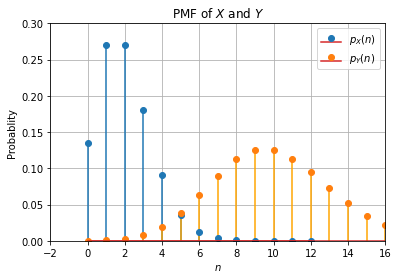
\includegraphics[width=0.85\columnwidth]{Figures/pmf_X_and_Y.png}
     \caption{$p_X(n)$ and $p_Y(n)$}
\end{figure}
    \end{frame}
\begin{frame}{Lemmas}
    \begin{lemma}[1]\label{lemma_X+Y}
        \vspace{-2mm}
        If $X$ and $Y$ are two independent Poisson distributions with parameters $\mu_1$ and $\mu_2$ respectively, then the distribution of $X+Y$ is also Poisson with parameter $\mu_1 + \mu_2$. 
    \end{lemma}
    \begin{block}{Proof.}
         We have for $k \geq 0$, the probability mass function $p_{X+Y}(k)$ is a convolution of pmfs $p_X(x)$ and $p_Y(y)$: \vspace{-2mm}
    \begin{align}
       p_{X+Y}(k) &= \pr{X+ Y = k} = \pr{Y = k - X}\\
       &= \sum_{i}\pr{Y = k - i| X=i}\times p_X(i)\label{p_(x+y)}
    \end{align}\vspace{-2mm}
    As X and Y are independent: \vspace{-1mm}
    \begin{align}
        \pr{Y\! =\! k - i \mid X=i} = \pr{Y\! = \! k - i} = p_Y(k-i)
    \end{align}\\\vspace{-3mm}
    \end{block}
\end{frame}
\begin{frame}{}
    \begin{proof}[Proof(Contd.)]
        Simplifying \eqref{p_(x+y)}\vspace{-2mm}
    \begin{align}
        p_{X+Y}(k) &= \sum_{i=0}^k p_Y(k-i) \times p_X(i)\\
        &= \sum_{i=0}^k e^{-\mu_2}\frac{\mu_2^{k-i}}{(k-i)!}e^{-\mu_1}\frac{\mu_1^i}{i!}\\
        &= e^{-(\mu_1 + \mu_2)}\frac 1{k!}\sum_{i=0}^k \frac{k!}{i!(k-i)!}\,\mu_1^i\,\mu_2^{k-i}\\
        &= e^{-(\mu_1 + \mu_2)}\frac 1{k!}\sum_{i=0}^k {k\choose i}\, \mu_1^i\,\mu_2^{k-i}\\
        p_{X+Y}(k) &= \frac{e^{-(\mu_1 + \mu_2)} \cdot (\mu_1 + \mu_2)^k}{k!}
    \end{align}
    \end{proof}
\end{frame}
\begin{frame}{}
    \begin{lemma}[2]\label{lemma_X-Y}
    \vspace{-2mm}
        If $X$ and $Y$ are two independent Poisson distributions with parameters $\mu_1$ and $\mu_2$ respectively, then the distribution of $X-Y$ is no longer Poisson, as $X - Y$ will also attain negative values.  More precisely, pmf of $X-Y$ is given by \eqref{pmf(X-Y)}, which is a Skellam distribution.
    \end{lemma}
    \begin{block}{Proof.}
         We have for $k \in \mathbb{Z}$, the probability mass function $p_{X-Y}(k)$ is a convolution of pmfs $p_X(x)$ and $p_Y(y)$: 
    \begin{align}
       p_{X-Y}(k) &= \pr{X\! -\! Y\! =\! k} = \pr{X\! =\! k\! +\! Y}\\
       &= \sum_{i}\pr{X = k + i| Y = i}\times p_Y(i)\label{p_(x-y)}
    \end{align}
    As X and Y are independent, and the Poisson distribution is zero for negative values of the count, the sum is only taken for those terms where $i \geq 0$ and $i+k\geq 0$.
    \end{block}
\end{frame}
\begin{frame}{}
\begin{block}{Proof(contd.)}
\vspace{-5mm}
\begin{align}
        p_{X-Y}(k) &= \sum_{i=max(0, -k)}^\infty p_X(k+i) \times p_Y(i)\\
        &=\sum_{i=max(0, -k)}^\infty e^{-\mu_1}\frac{\mu_1^{k+i}}{(k+i)!}e^{-\mu_2}\frac{\mu_2^i}{i!}\\
        &= e^{-(\mu_1 + \mu_2)}\sum_{i=max(0, -k)}^\infty \dfrac{\mu _{1}^{k+i}\mu _{2}^{i}}{i!(k+i)!}\label{pmf(X-Y)}
    \end{align}\\\vspace{-2mm}
    Hence we can see from \eqref{pmf(X-Y)} that X - Y is not a Poisson distribution.\\\qed
    
    \par \textbf{Note: } This result is valid only for independent Poisson distributions. We may have dependent Poisson distributions whose difference is also Poisson. For example let $Z$ be the random variable with distribution $X + Y$, where $X$ and $Y$ are independent Poisson distributions. From lemma (1), Z is Poisson. And, $Z - Y = X$ is also Poisson by definition, as $Z$ is always at least as great as $Y$ ($i.e.$ not independent).\\
    \end{block}    
\end{frame}
\begin{frame}{Solution}
    \begin{block}{Option 1}
        From the definition of Poisson process (Definition 1), $X$ and $Y$ are independent. Hence option 1 is \textbf{correct.}
    \end{block}
    \begin{block}{Option 2}
        As $X$ and $Y$ are independent Poisson distributions, using lemma (1), $X+ Y$ is a Poisson with parameter $\mu_1 + \mu_2 = 12 \neq 6$. Hence option 2 is \textbf{incorrect.}\vspace{-5mm}
    \begin{align}
         p_{X+Y}(k) &= \frac{e^{-(12)} \cdot (12)^k}{k!}\label{pmf(X+Y)}
    \end{align}
    \end{block}
    \begin{block}{Option 3}
        As $X$ and $Y$ are independent Poisson distributions, using lemma (2), $X-Y$ is not Poisson. Hence option 3 is \textbf{incorrect.}
    \end{block}
    \end{frame}
    \begin{frame}{}
\begin{figure}[h!]\label{graph_X-Y}
    \centering
      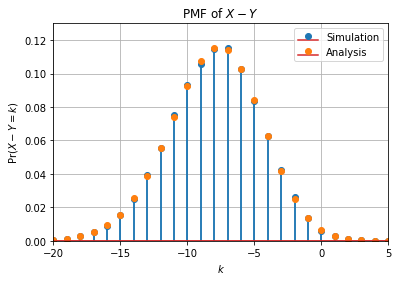
\includegraphics[width=0.85\columnwidth]{Figures/pmf(X-Y).png}
     \caption{$p_{X-Y}(k)$, with $\mu_1=2$ and $\mu_2=10$}
\end{figure}
    \end{frame}
    \begin{frame}
    \begin{block}{Option 4}\vspace{-4mm}
        \begin{align}
        \pr{X=0\mid X+Y=12} = \dfrac{\pr{X=0, Y=12}}{\pr{X+Y=12}}
    \end{align}
    As $X$ and $Y$ are independent, and using \eqref{pmf(X)}, \eqref{pmf(Y)}, and \eqref{pmf(X+Y)}, we have:
    \begin{align}
        \pr{X=0\mid X+Y=12} &= \frac{\pr{X=0} \cdot \pr{Y=12}}{\pr{X+Y=12}} \\
        &= \frac{\dfrac{e^{-2}\times 2^{0}}{0!} \times \dfrac{e^{-10}\times10^{12}}{12!}}{\dfrac{e^{-12}\times12^{12}}{12!}}\\
        &= \left(\dfrac{5}{6}\right)^{12}
    \end{align}
    Hence option 4 is \textbf{correct.}
    \end{block}
\textbf{Ans: (1), (4)}
\end{frame}
\end{document}
